We decided to implement first only a web user interface. This interface
is composed of one web-page developed in HTML 5 with some
pieces of JavaScript and CSS. We have taken care of having an
interface that fits nice on both huge screens of desktop computers
and small screens of phones.

\begin{figure}[!ht]
    \centering
    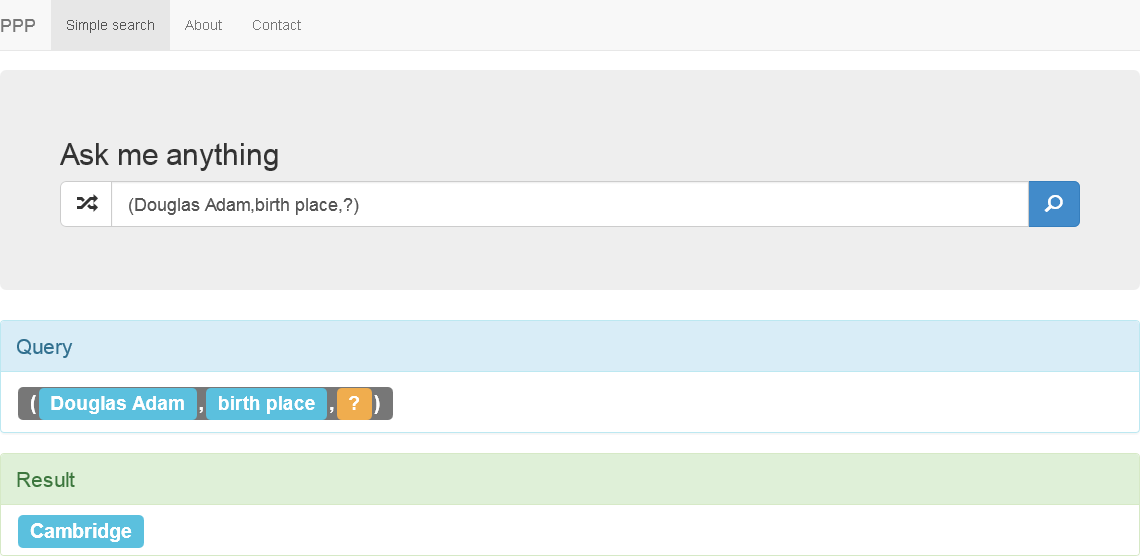
\includegraphics[scale=0.35]{WebUI.png}
    \caption{The user interface}
\end{figure}

It is composed of one huge text input with a button to submit
the query and another one to get a random question. The text area
allows both the input of questions in English or directly of triple using
an easy notation like \texttt{(Douglas Adam, birth date,?)} to find the
birth date of Douglas Adam. A small parser written in JavaScript converts
this easy to use notation into the standard format.

In order to build this interface we have relied on some famous libraries 
like \href{http://jquery.com/}{jQuery} and \href{http://getbootstrap.com/}{Bootstrap}.

\section{Logging}

We decided to log all requests made to the PPP to improve our algorithms,
and particularly to feed the results to Question parsing
modules that use Machine Learning.
We may also use it to improve the way the Core routes/sorts answers
from the different modules, either manually or with some basic
Machine Learning.

The main idea is to log user feedback in addition to the requests
themselves: after showing the user the way we interpreted their
question alongside the answer to their request, we provide them a
way to give us feedback.
What we call feedback is actually a thumb up / thumb down pair of
buttons, and, if the latter is pressed, a way to correct the requests
parsing result so it can be fed to the Machine Learning algorithms.

Since Machine Learning algorithms are not ready yet, we did not focus
on this feature of the user interface and thus it is not implemented yet;
so far we only started implemented a backend that stores data
(gathered via the user interface) to a SQLite database.
